\section{Design}

The system has been designed following a microservices architectural style, where each service models a specific subdomain and exclusively owns its data.

The principal objective of the design phase has been to:
\begin{itemize}
  \item ensure service autonomy.
  \item separate services persistence management.
  \item guarantee scalability and fault isolation.
  \item preserve local consistency while enabling eventual consistency across distributed services.
  \item separate responsibilities following domain partitioning.
\end{itemize}

A key design principle adopted is data ownership per service: no service directly accesses the database of another service.

All inter-service coordination occurs either synchronously or asynchronously.
This separation allows the system to tolerate partial failures, avoiding where possible cross-services synchronous operations chaining and maintain loose coupling among components.

\subsection{Structure}

The identification of domain entities and service boundaries has been guided by principles inspired by Domain-Driven Design (DDD).

The domain has been decomposed into bounded contexts, each representing a coherent business subdomain with its own model and behavior.

This approach has been adopted to:
\begin{itemize}
  \item reduce semantic ambiguity
  \item support independence between different subsystems
\end{itemize}

Each bounded context corresponds to a logically autonomous service, encapsulating:
\begin{itemize}
  \item domain entities
  \item business rules
  \item persistence layer
\end{itemize}

This alignment between domain boundaries and service boundaries reduces coupling and minimizes the need for distributed transactions, favoring asynchronous coordination and eventual consistency.

Given that, six bounded contexts are identified: user, event, interaction, chat, ticketing and notification.

Moreover, some other services are used: auth (Keycloak), media, payments (Stripe).

\subsubsection{Core Entities}

\begin{figure}[H]
  \centering
  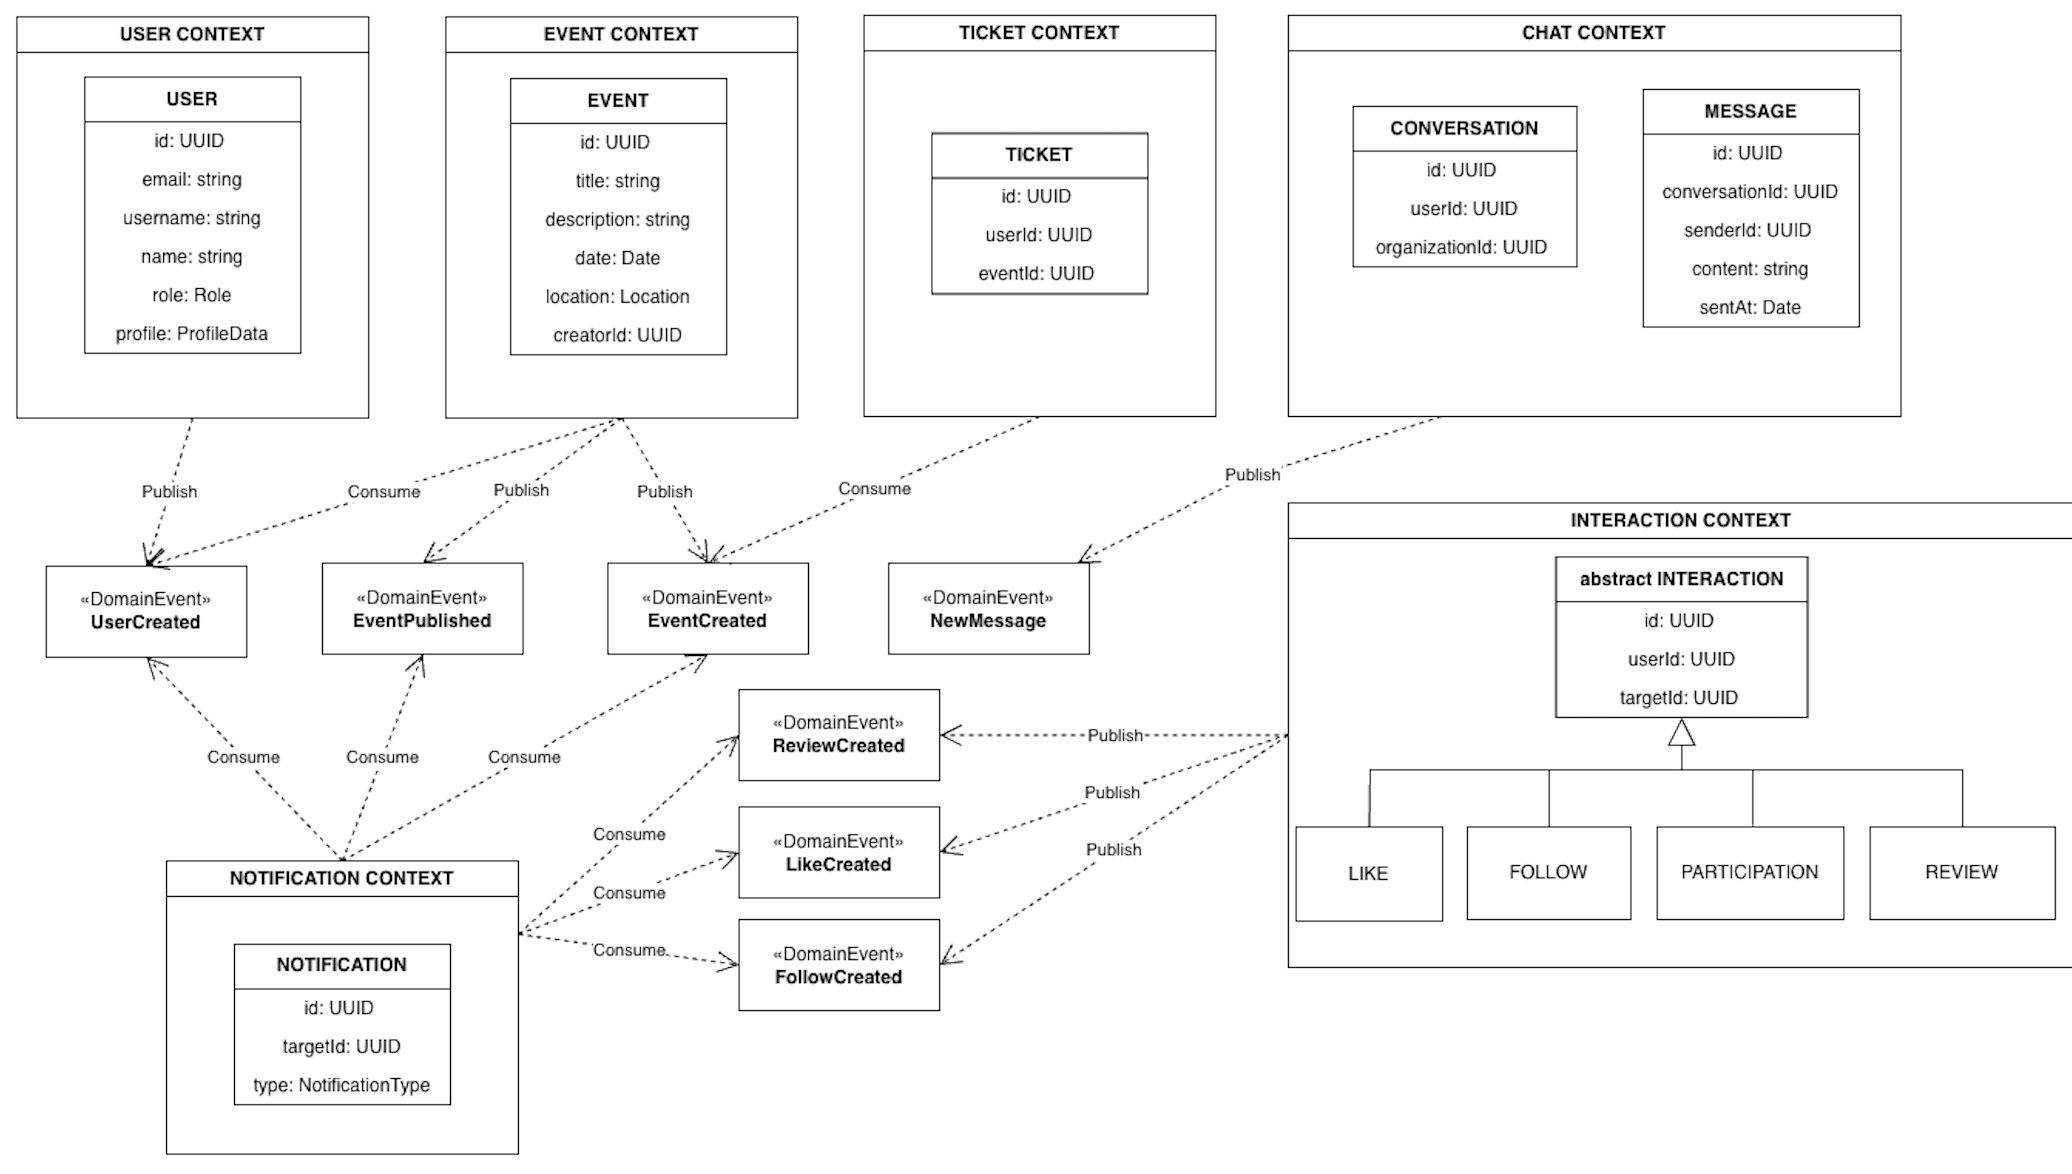
\includegraphics[width=\textwidth]{../public/core-entities.png}
  \caption{Core entities and bounded context diagram}
  \label{fig:core-entities}
\end{figure}

The diagram shows a simplification of the design, not every aspect of the model is represented in details.

The diagram highlights the separation between bounded contexts and the absence of direct structural dependencies across services.

Cross-service relationships are expressed through other entities identifier and domain events rather than object references or shared persistence.

\paragraph{User}
Represents a platform account.
A User can assume one of two roles:
\begin{itemize}
  \item Member
  \item Organization
\end{itemize}
Attributes include identifier, authentication-related data (account), profile information and events preferences.

\paragraph{Event}
Represents an activity created by an Organization.

Its attributes include identifier, title, description and all informations about event (e.g. date, time, location).

\paragraph{Ticket}
Represents a User's receipt of payment to participate in a Event.

It has its own lifecycle (creation, validation or invalidation) and is modeled independently from Event to avoid coupling financial logic with event management logic.

\paragraph{Interaction}

Abstract concept representing user actions.

In particular:
\begin{itemize}
  \item Like (User $\to$ Event)
  \item Follow (User $\to$ User)
  \item Review (User $\to$ Event)
  \item Participation (User $\to$ Event)
\end{itemize}

Interactions are separated from Event and User entities to enable event-driven propagation of user activities, allowing them to evolve independently from core domain entities.

\paragraph{Conversation}

Represents a communication channel between two Users. This entity stores information about the participants involved in the chat and metadata related to the conversation.

Messages are modeled as a separate entity rather than being embedded directly within the Conversation entity. This separation prevents unbounded data growth inside the conversation and allows message data to be managed independently.

Moreover, this design improves efficiency when retrieving the list of conversations. When a user requests the list of active conversations, the system only needs to access conversation metadata without loading all the associated messages. Message data is retrieved only when a specific conversation is opened.

\paragraph{Notification}

Represents a system-generated alert that must be sent to specific user.

Examples:
\begin{itemize}
  \item new follower
  \item new event published from followed organization
  \item new message/like/review received
\end{itemize}

Notifications are derived entities: they originate from domain events generated by other services.

\subsubsection{Domain Events}

In addition to static entities, the system models domain events to improve communication between services.

Examples include:
\begin{itemize}
  \item \texttt{UserCreated}
  \item \texttt{EventCreated}
  \item \texttt{EventPublished}
  \item \texttt{TicketPurchased}
  \item \texttt{LikeAdded}
  \item \texttt{NewMessage}
\end{itemize}

Domain events enable asynchronous integration between bounded contexts and allow the system to maintain eventual consistency.

\subsection{Interaction}

Communication between the different components of the system follows two interaction patterns: synchronous request--response and asynchronous event-based communication.

The choice of combining these two approaches allows the system to support direct user interactions while maintaining loose coupling and independent evolution of backend services.

\begin{itemize}
  \item \textbf{Synchronous interactions between frontend and backend services}:
  Synchronous communication is primarily used for interactions initiated by users through the frontend. In this pattern, a client sends a request to a service and waits for a response before continuing the execution.

  This approach is suitable for operations that require an immediate result, such as authentication, event browsing, or ticket purchasing. The response returned by the service confirms the successful execution of the operation or reports possible errors.
  Using synchronous interactions for user-driven operations simplifies the control flow and ensures that the user receives immediate feedback from the system.

  \item \textbf{Asynchronous event-driven communication}:
  Communication between backend services is primarily handled through asynchronous event-driven interactions. In this model, when a service completes an operation that may affect other parts of the system, it emits a domain event describing the change that occurred.
  Other services can subscribe to the events they are interested in and react accordingly. For example, the creation of an interaction or the publication of an event may trigger the generation of notifications or updates in other subsystems.
\end{itemize}

\paragraph{Consistency and coordination.}

Each service guarantees consistency within its own boundaries by executing state-changing operations within local transactions. After a transaction completes, the service may emit one or more domain events describing the resulting state change.

Other services process these events asynchronously, updating their own state or triggering additional operations. This approach avoids the need for distributed transactions across services and allows the system to maintain overall coherence through eventual consistency.

\subsection{Behaviour}

All of the services in the system follow a common behavioral structure when handling both user requests and inter-service communication.
The goal of this design is to maintain strong consistency within each service while enabling coordination between services in a distributed environment.

Three main behavioral patterns can be identified: request-driven operations, event-driven processing and real-time notification propagation.

\subsubsection{Request-Driven Operations}

User actions are processed through a request-driven workflow. A request is received by the API interface of the corresponding service and forwarded to the layer responsible for executing the domain logic.

To guarantee consistency, operations that modify the system state are executed within a local transactional boundary.

To guarantee reliability, it's adopted the \textbf{Outbox Pattern}. Instead of publishing events directly after the state update, domain events are first stored in a dedicated outbox structure within the same transaction as the database update. This ensures that the state change and the corresponding domain event recording occur atomically.
Once the transaction successfully completes, the events stored in the outbox can be asynchronously delivered to the message broker.

The typical workflow can therefore be summarized as follows:
\begin{enumerate}
  \item A client request is received through the service API.
  \item The request is validated and processed (optionally, also making synchronous request to other services) by the service logic.
  \item A local transaction updates the service state and if necessary records in the outbox the domain events describing the change.
  \item After the transaction completes, the events are asynchronously published.
\end{enumerate}

This pattern guarantees internal consistency within the service while enabling reliable propagation of domain events to the rest of the system.

\begin{figure}[H]
  \centering
  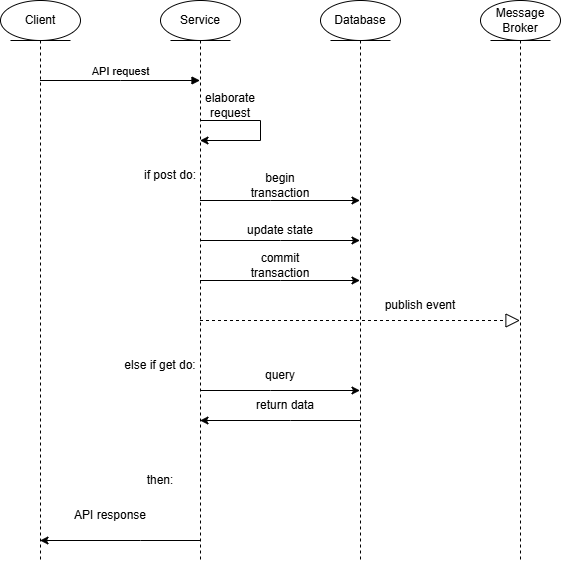
\includegraphics[width=0.7\textwidth]{../public/design/behavior-request-driven.png}
  \caption{Request-driven behavior}
  \label{fig:behavior-request-driven}
\end{figure}

\subsubsection{Event-Driven Processing}

Services also react to domain events generated by other services.
When an event is received, the service processes it through its domain logic and may update its internal state or trigger additional events.

This approach enables coordination between bounded contexts without requiring direct dependencies between services.

The typical flow for this interaction is:
\begin{enumerate}
  \item A domain event is received.
  \item The service processes the event through its domain logic.
  \item If required, a local transaction updates the service state.
  \item Additional domain events may be generated.
\end{enumerate}

This event-driven approach allows services to collaborate asynchronously while preserving loose coupling and independent evolution.

\begin{figure}[H]
  \centering
  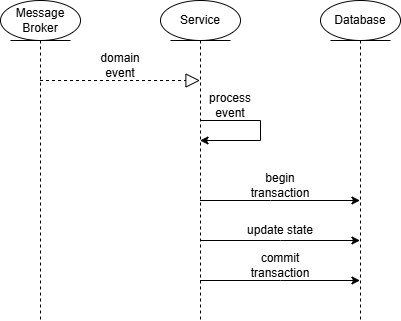
\includegraphics[width=0.7\textwidth]{../public/design/behavior-event-driven.png}
  \caption{Event-driven behavior}
  \label{fig:behavior-event-driven}
\end{figure}

\subsubsection{Real-Time Notification Propagation}

A specific behavior is implemented for real-time user notifications.
Some domain events represent user actions that must be sent to other users, such as a message or a new interaction. These events trigger the creation of notification entities.

The notification subsystem processes the relevant events, stores the corresponding notification and propagates it to connected clients through a real-time communication channel.

The workflow is the following:
\begin{enumerate}
  \item A domain event is generated by a service.
  \item The notification subsystem consumes the event.
  \item A notification entity is created and stored.
  \item The notification is delivered to relevant connected clients in real-time.
\end{enumerate}

This mechanism allows the system to react promptly to user-relevant events while maintaining a decoupled architecture.

\begin{figure}[H]
  \centering
  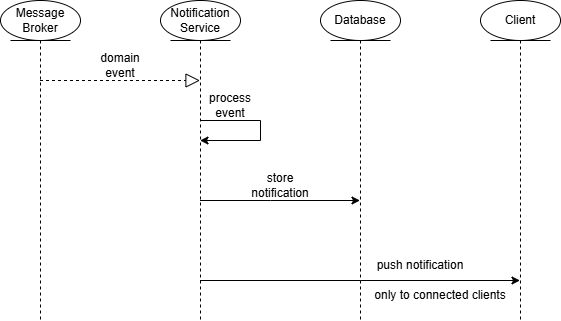
\includegraphics[width=\textwidth]{../public/design/behavior-real-time.png}
  \caption{Real-time notification propagation behavior}
  \label{fig:behavior-real-time}
\end{figure}

\subsection{Architecture}

\subsubsection{Architectural Style}

The system is designed according to a \textbf{microservices architecture}. The application is decomposed into a set of small, independently deployable services, each responsible for a specific bounded context: user, event, interaction, chat, ticketing and notification.

Each microservice encapsulates its own domain logic and adopts the \textbf{database-per-service} pattern.

When shared information is required (e.g., basic user data such as \texttt{id}, \texttt{name} and \texttt{avatar} needed by the \texttt{chat} or \texttt{interaction} services), it is propagated via \textbf{domain events} rather than retrieved through synchronous queries. This intentional data duplication reduces communication overhead and keeps services decoupled.

Moreover, this design avoids the bottleneck that would arise from sharing a single database across multiple services and guarantees strong data ownership by preventing services from directly accessing another service's data store.
\newpage
\noindent\textbf{Inter-service communication}

Two complementary communication styles are adopted:

\begin{itemize}
  \item \textbf{Synchronous (HTTP REST)}: used when fulfilling a request requires invoking an operation or retrieving data from another service, or to propagate state changes immediately to dependent services. For example, when an event is created, the \texttt{event} service notifies \texttt{ticketing} via its internal API so that ticket-related operations can proceed right away.

  \item \textbf{Asynchronous}: used to propagate state changes across service boundaries without creating runtime dependencies between them and to push real-time updates to connected clients. Three mechanisms are in place:
    \begin{itemize}
      \item \textbf{Domain events (RabbitMQ)}: services publish events to the message broker; subscribers consume them independently. For example, when an event is published, the \texttt{event} service emits an \texttt{EventPublished} domain event consumed by the \texttt{notification}, \texttt{ticketing} and \texttt{interaction} services.
      \item \textbf{WebSocket (Socket.IO)}: used by the \texttt{notification} service to maintain persistent connections with clients, enabling server-side push of real-time updates without polling. For example, when \texttt{notification} receives an \texttt{EventPublished} domain event, it delivers an update to the relevant connected clients. In this case, users following the organization that published the event.
      \item \textbf{Webhooks}: used for third-party integrations that push notifications into the system, for example payment provider (Stripe) callbacks delivered to the \texttt{ticketing} service. The receiving service processes the incoming HTTP call asynchronously without blocking any client-facing request.
    \end{itemize}
\end{itemize}

\noindent\textbf{API gateway}

All external traffic flows through an API gateway implemented with \textbf{Traefik}, which acts as a single entry point and keeps the internal service topology invisible to clients.

\medskip
\noindent\textbf{Motivation for the architectural choice}

\begin{itemize}
  \item \textbf{Service independence}: each service can be developed, tested and deployed independently.
  \item \textbf{Scalability}: services can scale horizontally according to their specific load.
  \item \textbf{Loose coupling}: the combination of database-per-service and event-driven communication minimises direct dependencies, improving maintainability.
  \item \textbf{Data isolation}: each service's database schema evolves independently, preventing unintended cross-service coupling.
  \item \textbf{Resilience and fault isolation}: failures are contained within individual services; asynchronous communication through the message broker allows a service to be temporarily unavailable without blocking the rest of the system.
\end{itemize}

\subsubsection{Infrastructure}

\begin{figure}[H]
  \centering
  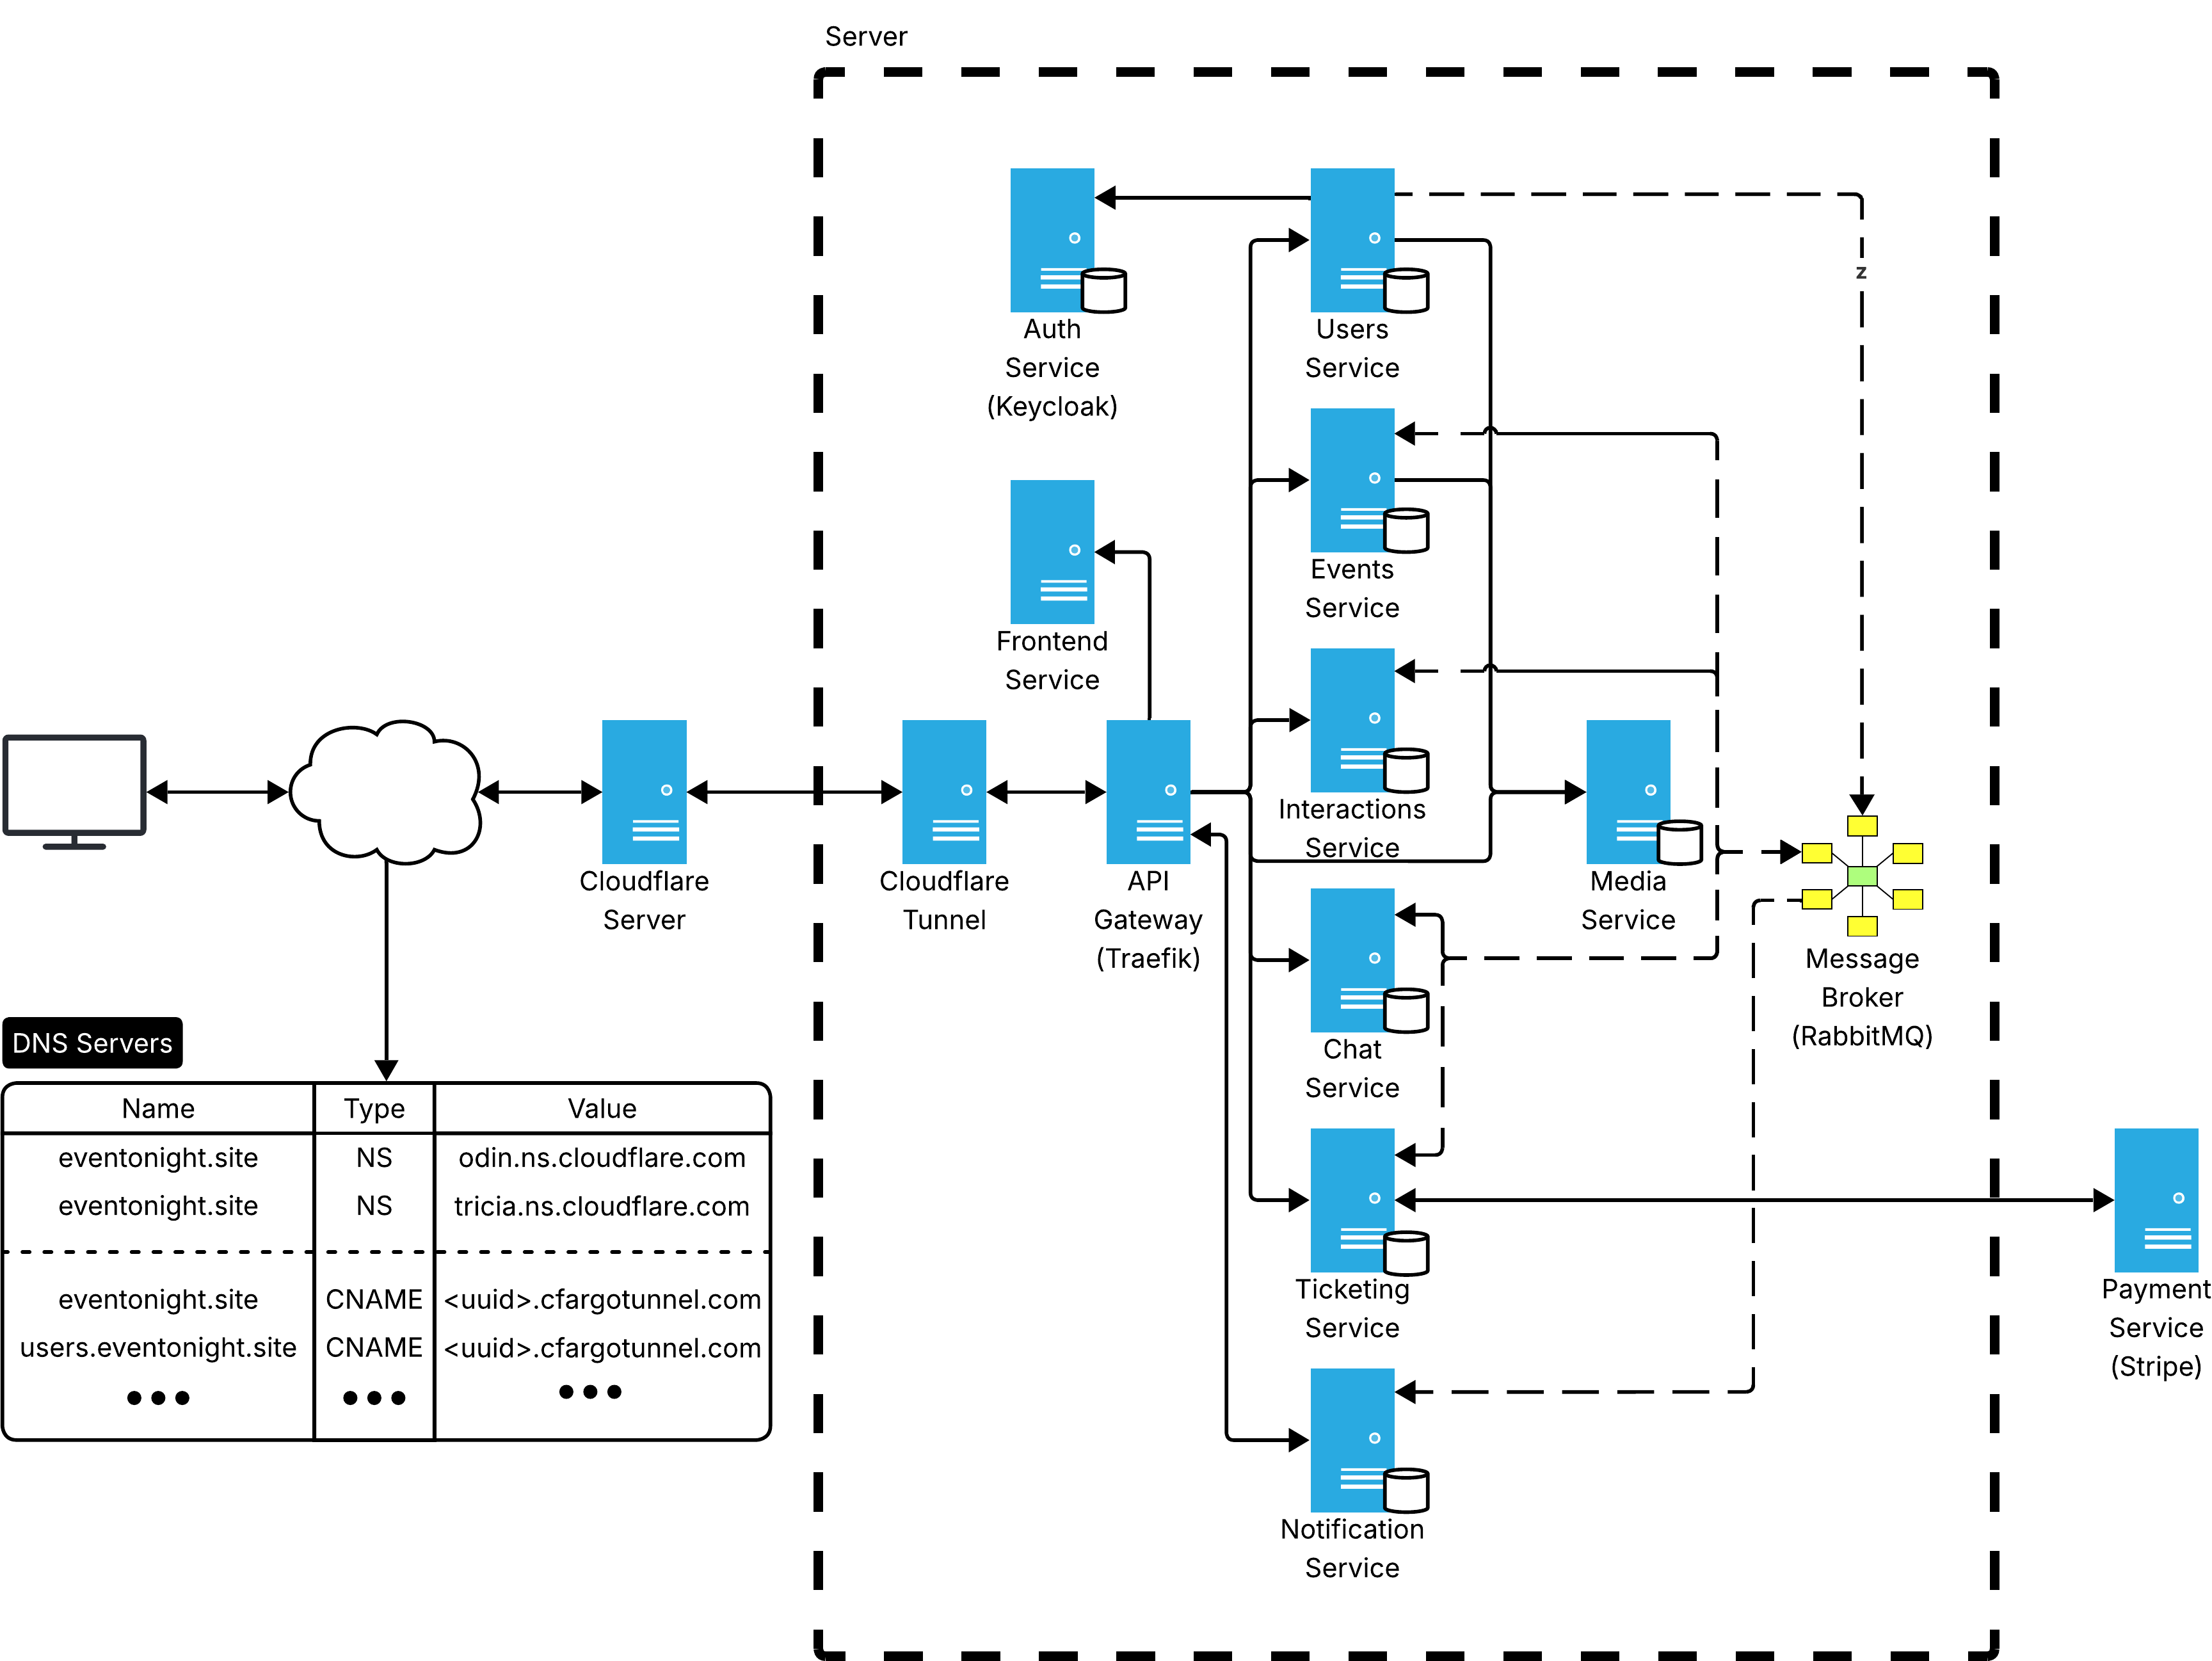
\includegraphics[width=\textwidth]{../public/design/Infrastructure.png}
  \caption{Infrastructure diagram}
  \label{fig:infrastructure}
\end{figure}
\newpage
\noindent\textbf{Components}

All infrastructural components are listed in the table below.

\begin{table}[H]
  \centering
  \begin{tabular}{p{3.2cm}p{3.2cm}p{7cm}}
    \toprule
    \textbf{Component} & \textbf{Technology} & \textbf{Description} \\
    \midrule
    DNS / TLS & Cloudflare & Authoritative DNS and TLS termination \\
    Tunnel daemon & cloudflared & Maintains an outbound encrypted tunnel to Cloudflare; no inbound ports required on the cluster \\
    API gateway / Reverse proxy & Traefik v3 & Single entry point for all external HTTP/WebSocket traffic; handles routing, load balancing, rate limiting, retries, circuit breaking and request timeouts; discovers services via Docker label-based configuration \\
    Backend services & Scala 3 + Cask & \texttt{user}, \texttt{event} \\
    Backend services & NestJS (Node.js) & \texttt{chat}, \texttt{interaction}, \texttt{ticketing} \\
    Backend services & Express (Node.js) & \texttt{media}, \texttt{notification} \\
    Frontend & Vue 3 + Vite & Single-page application served as static assets \\
    Identity provider & Keycloak & User authentication and JWT issuance \\
    Message broker & RabbitMQ & Asynchronous event delivery via a topic exchange \\
    Document databases & MongoDB & One dedicated instance per service \\
    Relational database & PostgreSQL & Backing store for Keycloak \\
    Object storage & MinIO & Binary file and image storage for the \texttt{media} service \\
    Payment provider & Stripe \textit{(external)} & Third-party payment processing \\
    Seed service & Node.js & Populates databases with initial data on first deployment \\
    \bottomrule
  \end{tabular}
  \caption{Infrastructure components}
  \label{tab:infrastructure}
\end{table}

\noindent\textbf{Network distribution}

With the exception of Stripe, all components run inside a single host using \textbf{Docker Compose}. No service port is exposed to the public internet, the only inbound path is through the Cloudflare tunnel.

Two categories of Docker bridge networks are used:

\begin{itemize}
  \item \textbf{\texttt{eventonight-network}}: shared by all application services, Traefik, RabbitMQ and Keycloak. Used for inter-service communication and Traefik routing.
  \item \textbf{\texttt{<service>-network}}: one private network per service, shared exclusively between the service, its database instance and any auxiliary containers (e.g. provisioning scripts that perform initial setup, as in the case of Keycloak). This enforces database isolation, no other service can reach another service's database.
\end{itemize}

\noindent\textbf{Service discovery}

External clients resolve subdomains through Cloudflare's authoritative DNS. Each subdomain is a CNAME record pointing to \texttt{<uuid>.cfargotunnel.com}, which resolves to a Cloudflare edge IP. Traffic enters the cluster through the \texttt{cloudflared} tunnel and is handed off to Traefik.

Inside the host, discovery is handled by Docker Compose:

\begin{itemize}
  \item \textbf{Internal DNS}: Compose registers each service by name in the internal DNS (e.g., \texttt{http://users:9000}, \texttt{amqp://rabbitmq:5672}). No manual registration is required.
  \item \textbf{Traefik routing}: Traefik watches the Docker API for label changes and rebuilds its routing table automatically when services are started or stopped.
\end{itemize}

\subsubsection{Data Flow}

\noindent\textbf{Synchronous request flow (HTTP REST)}

\begin{verbatim}
Browser → Cloudflare (DNS + TLS) → cloudflared
        → Traefik → Service → Database → response
\end{verbatim}

The browser sends an HTTPS request to a subdomain (e.g., \texttt{events.eventonight.site}). Cloudflare resolves the DNS and terminates TLS, then injects the request into the persistent encrypted tunnel (QUIC) maintained by \texttt{cloudflared} on the cluster. Traefik receives it, matches the \texttt{Host} header against its routing rules and forwards the request to the target service. The service handles the request, queries its own database instance and returns the response through the same chain.

\medskip
\noindent\textbf{Asynchronous event flow (AMQP)}

\begin{verbatim}
Service → Exchange (eventonight) → Queue (per-service) → Consumer service
\end{verbatim}

\begin{figure}[H]
  \centering
  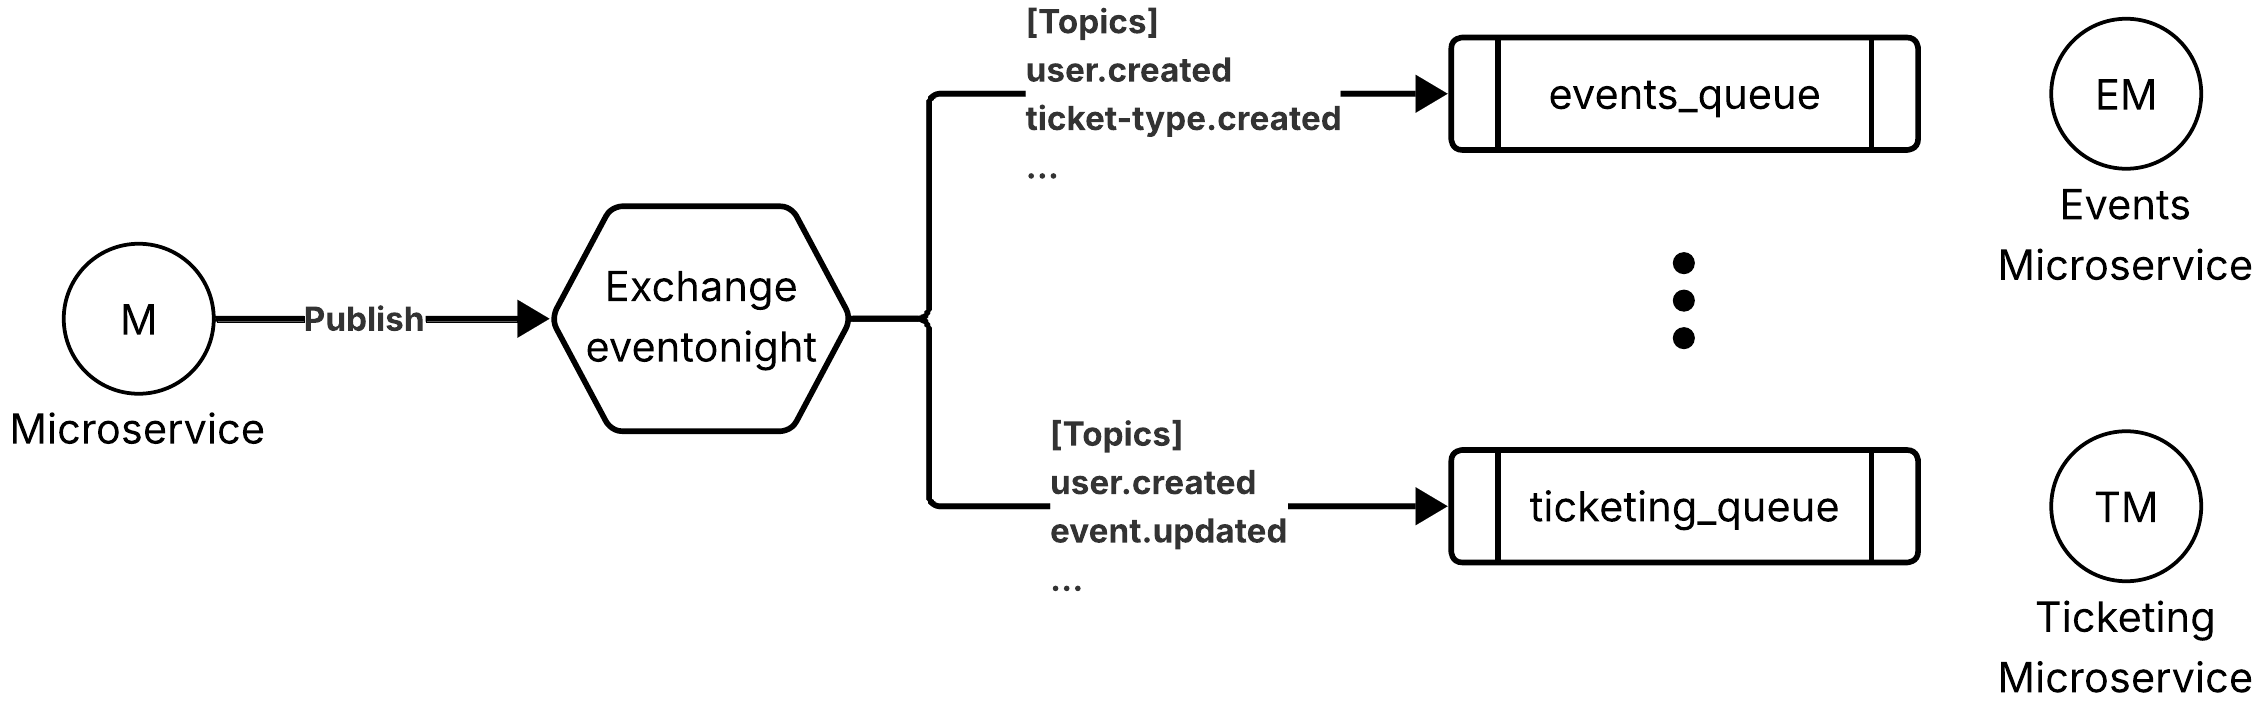
\includegraphics[width=\textwidth]{../public/design/Broker.png}
  \caption{Message broker topology}
  \label{fig:broker}
\end{figure}

RabbitMQ uses a single \textbf{topic exchange} named \texttt{eventonight}. Each consuming service has a dedicated queue bound to the exchange with a set of topic subscriptions (e.g., \texttt{ticketing\_queue} binds to \texttt{user.created}, \texttt{event.updated} and many others). When a service publishes a domain event with a routing key, the exchange fans it out to every queue whose binding pattern matches, without the publisher knowing who the consumers are.

\newpage
\noindent\textbf{Real-time push (WebSocket)}

\begin{verbatim}
notification service → Socket.IO → Browser
\end{verbatim}

The \texttt{notification} service consumes events from its queue and pushes real-time updates to the relevant connected clients over WebSocket (Socket.IO).

\medskip
\noindent\textbf{Webhook flow (Stripe $\to$ ticketing)}

\begin{verbatim}
Stripe → Cloudflare → cloudflared → Traefik
       → ticketing (acknowledged immediately, processed asynchronously)
\end{verbatim}

Stripe delivers payment event callbacks via HTTP POST to the \texttt{ticketing} service. The service responds immediately with \texttt{200 OK} and processes the event asynchronously, without blocking any client-facing operation.

\subsubsection{Web API}

All application services expose a \textbf{REST API}, accessible externally via Traefik at \texttt{<service>.even\allowbreak tonight.site}. Every protected endpoint requires a \textbf{JWT Bearer token} in the \texttt{Authorization} header, issued by Keycloak and validated independently by each service using Keycloak's public key, no centralised auth gateway is needed.
The \texttt{notification} service additionally exposes a \textbf{WebSocket endpoint}.

\subsubsection{Scalability and High Availability}

The current deployment runs all components on a \textbf{single host} using Docker Compose. Each service runs as a single container instance, which provides basic availability but represents a single point of failure at the host level.
The architecture below is designed to transition to \textbf{high availability} by adopting \textbf{Docker Swarm}.

\begin{figure}[H]
  \centering
  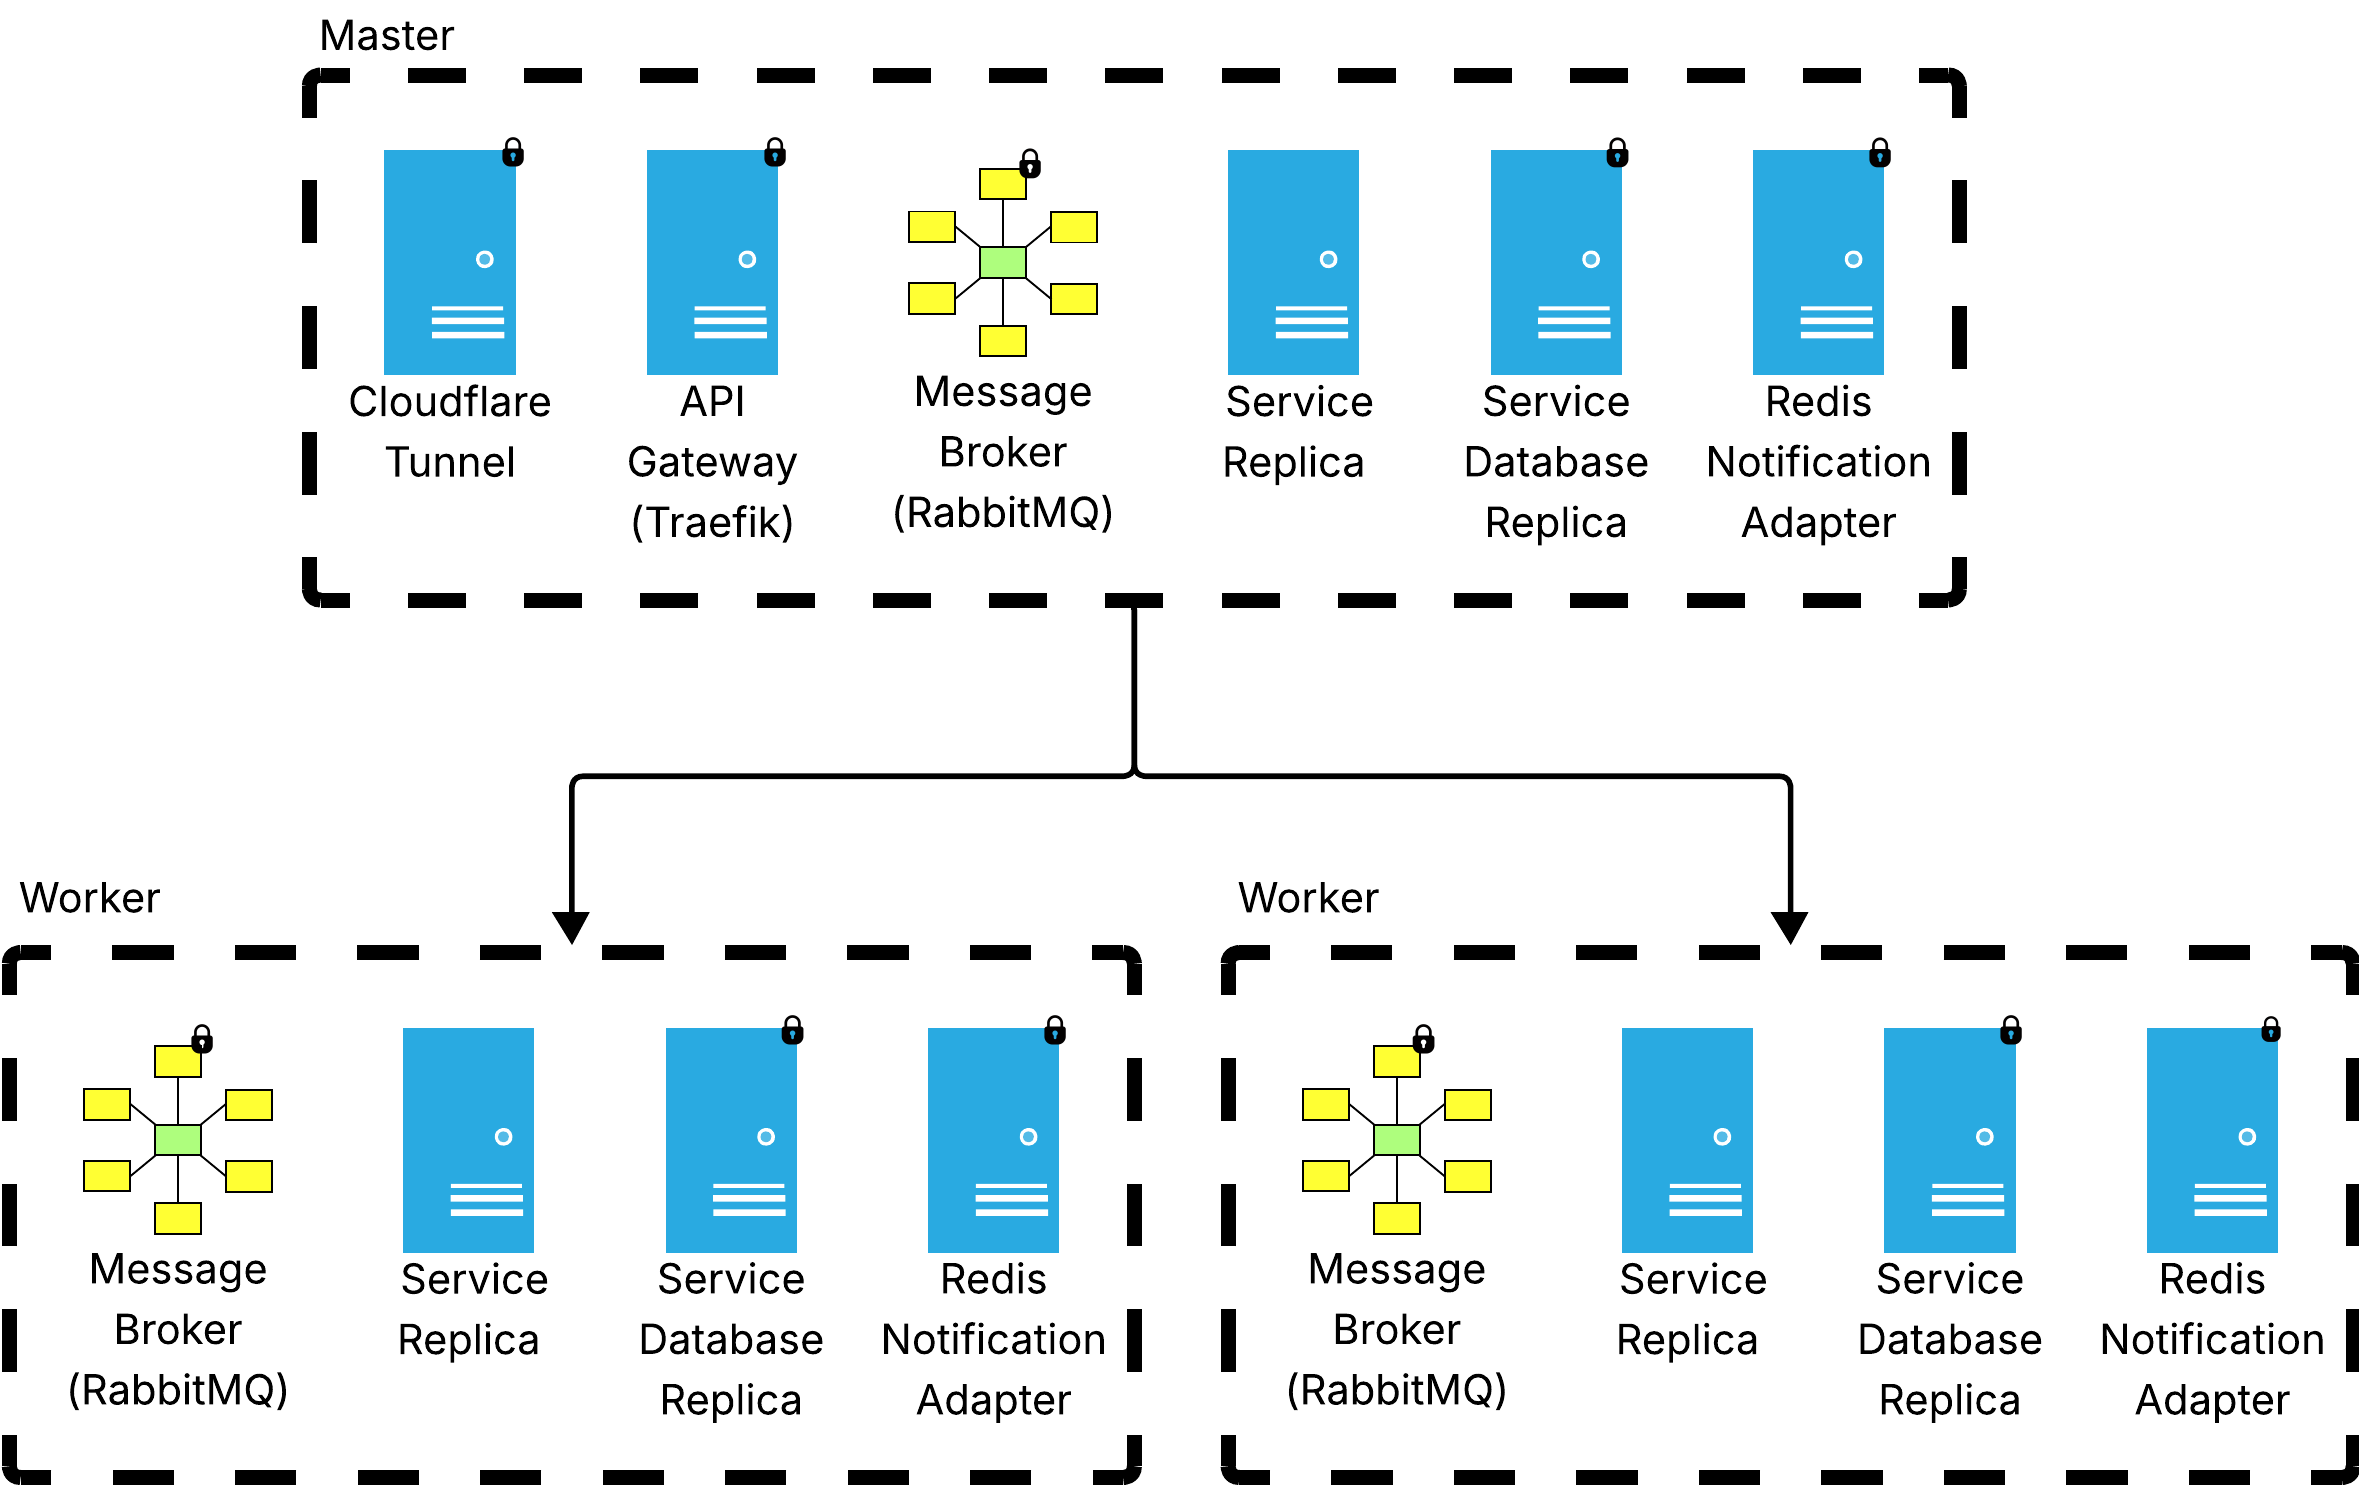
\includegraphics[width=0.9\textwidth]{../public/design/Swarm.png}
  \caption{Docker Swarm deployment topology}
  \label{fig:swarm}
\end{figure}

Even on a single node, Swarm already provides a first step toward HA through \textbf{rolling updates}, services can be updated replica by replica with zero downtime, unlike a plain Compose deployment where an update implies a brief interruption. Moving to a multi-node cluster then enables true HA by distributing replicas across machines, so that the failure of a node does not take down the service.

However, adding nodes and replicas is a necessary but not sufficient condition for HA, it also requires deliberate design choices at the infrastructure level and at the application level to preserve correctness: stateful services require dedicated replication strategies and deploying multiple replicas of a service introduces competing consumer scenarios on the broker that must be explicitly handled.

\medskip
\noindent\textbf{Cluster topology}

For true HA, the Swarm should have at least \textbf{three manager nodes}. Swarm managers use the Raft consensus protocol to maintain cluster state and an odd number of managers is required to form a quorum and tolerate node failures (three managers tolerate one failure). Each manager node should run its own Traefik and \texttt{cloudflared} instance, so Cloudflare load-balances incoming traffic across all managers automatically.

\medskip
\noindent\textbf{Service placement}

Stateless application services can be freely distributed across nodes. Stateful services (RabbitMQ and databases) require \textbf{placement constraints} to be distributed and binded on different machines. Manager nodes should be set to \textbf{drain} availability so the Swarm scheduler assigns no application workloads to them, keeping them dedicated exclusively to cluster management and incoming traffic.

\medskip
\noindent\textbf{Message broker with multiple consumers}

Scaling application services to multiple replicas introduces a non-trivial consideration for broker consumption. The current setup uses a \textbf{single active consumer} per queue: only one replica consumes from a given queue at a time, guaranteeing FIFO message processing. This is sufficient for HA because if the active consumer fails, another replica takes over, but it does not improve throughput.

To scale throughput beyond a single consumer, more refined strategies can be explored:

\begin{itemize}
  \item \textbf{Consistent hash exchange}: a RabbitMQ plugin that replaces the standard topic exchange with a hashing layer. Using that, messages are routed to one of N queues based on a hash of the routing key, allowing N consumers to process in parallel while preserving per-key ordering.
  \item \textbf{Streams / Super Streams}: RabbitMQ Streams provide a persistent, replayable log. Super Streams partition a logical stream across multiple physical streams, each consumed by a dedicated replica, combining throughput scaling with ordering guarantees per partition.
  \item \textbf{Sequence fields}: adding a monotonically increasing \texttt{version} or \texttt{seq} field per entity allows consumers to detect and discard out-of-order messages regardless of the consumption strategy adopted.
\end{itemize}

\noindent\textbf{What changes with Swarm:}

\begin{itemize}
  \item \textbf{\texttt{cloudflared} and Traefik} scale with the number of manager nodes, one instance per manager. Traefik natively supports Swarm mode via the Docker API.
  \item \textbf{Stateless application services} can be scaled to multiple replicas and distributed freely across nodes.
  \item \textbf{Stateful services} require dedicated HA strategies: MongoDB moves to a \textbf{replica set} (primary + secondaries) and RabbitMQ to a \textbf{quorum queue cluster}, both require an odd number of members (e.g. 3, 5) to guarantee quorum and avoid split-brain, ensuring data redundancy and automatic failover. Each stateful instance must be pinned to a distinct node (at most one replica per node) so that a single node failure does not take down multiple members of the same cluster. Replicated data stores also improve \textbf{fault tolerance}, the system continues to operate and preserves data integrity even if individual nodes are lost.
  \item \textbf{WebSocket sticky sessions}: when \texttt{notification} runs as multiple replicas, Traefik must be configured with a sticky cookie to ensure Socket.IO handshake and subsequent frames are consistently routed to the same replica. However, sticky sessions alone are not sufficient: to broadcast events to all connected clients regardless of which replica they are connected to, a \textbf{Redis adapter} for Socket.IO is required to propagate messages across all instances.
\end{itemize}

\subsection{Corner Cases}

The system is designed to be \textbf{highly available} and \textbf{eventual consistent}. Each service operates independently and failures are isolated: when a component goes down, only the functionality directly depending on it is affected, while the rest of the system continues to operate.

\paragraph{Fault detection.}
Each service exposes a \texttt{/health} endpoint and declares a \texttt{healthcheck} in Docker Compose. This allow Docker to automatically restarts or reschedules tasks that become unhealthy, making fault detection active. To further improve observability, a dedicated monitoring service could be introduced.

\paragraph{Startup ordering and reconnection.}
In a Compose deployment, dependent services use \texttt{depends\_on} with \texttt{condition: service\_healthy} to enforce startup ordering. In a Swarm deployment this mechanism is not available: each service must instead be resilient to the temporary unavailability of its dependencies and implement reconnection logic autonomously. Note that reconnection logic is necessary regardless of the deployment model, as dependencies may also fail and recover during normal operation. All reconnection attempts, to MongoDB, RabbitMQ and other services, use an exponential backoff strategy.

\paragraph{Error signalling.}
Every API endpoint returns standard HTTP status codes to communicate failures to clients: \texttt{400} for validation errors, \texttt{401} for missing or invalid tokens, \texttt{403} for authorisation failures, \texttt{404} for resources not found, \texttt{409} for conflicts, \texttt{500} for unexpected server errors and so on. With a monitoring service in place, an alerting mechanism can be added to proactively notify on service failures.

\paragraph{Component failure and recovery.}
In a Compose deployment, all containers run with \texttt{restart: unless-stopped}, so Docker automatically restarts any crashed container. Docker itself is configured to start on host boot, meaning that even a full machine reboot brings the entire system back up without manual intervention. In a Swarm deployment, the restart policy is managed by the Swarm scheduler, which restarts failed tasks and, if a node goes down, reschedules its tasks onto healthy nodes automatically. In both cases, full recovery is achieved because services are resilient to dependency failures and re-establish connections autonomously.

\paragraph{Database failure.}
If a MongoDB instance goes down, its owning service remains partially operational: requests that do not require the database can still be served. The service reconnects automatically when the database comes back up. In a Swarm deployment with a replica set, a single node failure triggers an automatic primary election and the service reconnects to the new primary, avoiding a full outage. In both cases, multi-document operations are executed within MongoDB transactions, so a crash mid-operation leaves no inconsistent state, the transaction is simply rolled back.

\paragraph{Service failure.}
If a service crashes, Docker restarts it automatically. Since all writes are transactional, there is no risk of partial state being committed. However when a service crashes after initiating an outbound HTTP call to an external system (e.g. creating a Stripe checkout session or a Keycloak user) but before completing its local operations, an inconsistency may arise: the side effect on the external system has already occurred but the local state does not reflect it. In these cases specific strategy must be applied for each integration to handle it correctly.

\paragraph{RabbitMQ failure.}
All queues are declared as durable with persistent messages, so any message received by RabbitMQ before it goes down is safely stored to disk and delivered to consumers once it restarts. In a Swarm deployment with a quorum queue cluster, a single node failure does not cause an outage, the cluster continues operating as long as a majority of nodes are available and messages are replicated across them. RabbitMQ provides at-least-once delivery semantics; services handle this by designing message handlers to be idempotent. If RabbitMQ is unavailable at the moment a service needs to publish, messages are not lost since each service implements the outbox pattern.

\paragraph{Keycloak failure.}
If Keycloak goes down new logins and token refreshes will fail. However, services validate JWTs locally using Keycloak's public key, so requests carrying a still-valid token continue to be accepted until expiry. Once Keycloak restarts, authentication resumes normally.

\paragraph{Traefik or cloudflared failure.}
In a Compose deployment, external traffic cannot enter the system until Docker restarts the container and access resumes. In a Swarm deployment, both run one instance per manager node, so a single manager failure does not interrupt external traffic, Cloudflare simply routes through the remaining instances.

\paragraph{Ticketing crash during checkout session creation.}
If \texttt{ticketing} crashes after tickets have been reserved and the Stripe session has been created, but before send response to the client, the session will eventually expire and Stripe delivers a \texttt{checkout.session.expired} webhook allowing \texttt{ticketing} to release the reserved tickets. If the crash occurs before the Stripe session is created, no webhook will ever arrive and the tickets remain stuck in \texttt{PENDING}; a background cleanup job on timed-out pending orders would be needed to handle this case.

\paragraph{Ticketing unavailability.}
Webhook callbacks from Stripe cannot be processed. Stripe automatically retries undelivered events for up to three days, so the \texttt{ticketing} service will receive and process them once it recovers, without any data loss.

\paragraph{Dual notification path (sync + async).}
When an event is created, the \texttt{event} service notifies \texttt{ticketing} synchronously via HTTP call to an internal endpoint, without waiting for the asynchronous domain event to arrive. The RabbitMQ message still follows as a fault-tolerance fallback.

\paragraph{User crash during register and password update.}
If \texttt{user} crashes after creating the account in Keycloak but before persisting the user record locally, the user exists in the identity provider but not in the \texttt{user} service. On the next login attempt, Keycloak authenticates the user and issues a valid JWT, but \texttt{user} has no matching record. A recovery strategy can be to detect this condition at login time and create a minimal empty profile automatically, mirroring what registration would have done. For password updates, a crash mid-operation leaves the state consistent but the user may not have been correctly notified of the outcome; a "forgot password" flow provides a user-friendly self-service recovery path in this case.

\paragraph{Consistent backup.}
Because each service owns its own database, there is no single point from which to take a globally consistent snapshot. Backing up each database independently means the captured states may be at slightly different points in time. Full cross-service consistency at backup time is not achievable without a distributed snapshot protocol. One practical mitigation is to temporarily halt writes across all services, snapshot all databases simultaneously, then resume, guaranteeing consistency at the cost of a short downtime.
